% ch-introduction.tex -- what Yuzen is and what it is for
\chapter{Introduction}
\label{ch:introduction}

Yuzen computes how a thin liquid layer on a substrate evolves in time: how it
levels under surface tension, how it is driven by gravity and rotation, how the
solvent evaporates so that the film thickens and eventually stops flowing, and
how the contact line at its edge advances or recedes.

It is a research solver, written in C++17, with no dependency you have to
install by hand. You describe a case in one text file, run one executable, and
get a directory of results that opens in ParaView.

\section{What Yuzen solves}
\label{sec:intro:what}

Yuzen solves the long-wave (lubrication) equation for the film height
$h(x,y,t)$, coupled to a transport equation for the solute concentration
$c$. In dimensionless form,
%
\begin{align}
  \frac{\partial H}{\partial T} &= -\nabla\cdot\Qvec - \Ev\,\hat{E}(H,C) + \hat{S},
  \label{eq:intro-height}\\
  \frac{\partial (HC)}{\partial T} &= -\nabla\cdot\bigl(C\,\Qvec\bigr)
    + \Df\,\nabla\cdot\bigl(\hat{D}(C)\,H\,\nabla C\bigr) + C_S\,\hat{S},
  \label{eq:intro-conc}
\end{align}
%
where the flux $\Qvec$ collects capillary leveling, disjoining pressure,
vertical and in-plane gravity, centrifugal force and the Marangoni stress.
The first equation moves the liquid; the second moves the solute $HC$ with the
same flux and lets it diffuse, and evaporation, which takes solvent only, is
absent from it --- it concentrates the solute by thinning the film. The liquid
$\hat{S}$ a nozzle supplies brings solute at the concentration $C_S$ it
arrives at: the local $C$ by default, or a concentration of its own. The full
forms are derived in \cref{ch:governing}, each term is discussed in
\cref{ch:terms}, and \cref{ch:concentration} adds a model that resolves $C$
through the thickness.

The approximation behind \cref{eq:intro-height} is that the film is thin
compared with the in-plane length over which it varies. That single assumption
reduces the Navier--Stokes equations to one evolution equation for $h$, which
is what makes it possible to compute a whole coated wafer rather than a few
millimeters of one. It also sets the limits of the model, and
\cref{sec:governing:breakdown} states them explicitly rather than leaving you
to discover them.

\section{Physical processes}
\label{sec:intro:physics}

Each process below is a separate term of the equations, switched on by its
own block of the input file (\cref{ch:ref-physics}); a block left out means
that term is off.

\begin{itemize}
  \item Capillary (Laplace) pressure: leveling by surface tension
    (\cref{sec:terms:laplace}).
  \item Disjoining pressure: wetting, dewetting and a moving contact line on a
    precursor film, calibrated to an equilibrium contact angle
    (\cref{sec:terms:disjoining}, \cref{ch:wetting}).
  \item Vertical gravity, including flow over a non-flat substrate
    (\cref{sec:terms:vgravity}).
  \item In-plane gravity: drainage on an inclined substrate
    (\cref{sec:terms:hgravity}).
  \item Centrifugal force: spin coating (\cref{sec:terms:centrifugal}).
  \item Solutal Marangoni stress (\cref{sec:terms:marangoni}).
  \item Navier slip at the substrate (\cref{sec:terms:slip}).
  \item Solvent evaporation, with spatial profiles and a correction on the
    precursor film (\cref{sec:terms:evaporation}).
  \item Liquid supplied by a fixed or moving nozzle (\cref{sec:terms:source}).
  \item Solute transport, well mixed through the thickness or resolved across
    it, with viscosity, surface tension and diffusivity depending on the
    concentration (\cref{ch:concentration}).
\end{itemize}

\section{What it is good for}
\label{sec:intro:uses}

Typical applications are spin-coated photoresist, functional coatings, drying
films, and wetting and dewetting problems. Concretely, Yuzen is a reasonable
choice when

\begin{itemize}
  \item the film is thin compared with the in-plane features you care about,
        so that $\As = (L_0/h_0)^2$ is large;
  \item the flow is viscous and inertia is negligible;
  \item you need the film shape over seconds to minutes of physical time,
        rather than the three-dimensional velocity field at one instant;
  \item the interesting physics is some combination of leveling, drying,
        Marangoni streaking, spinning and contact-line motion.
\end{itemize}

It is the wrong tool when inertia matters, when the interface slope is large
everywhere rather than only near the contact line, when the film breaks up into
droplets that separate, or when you need the flow inside the film in three
dimensions. \Cref{sec:governing:breakdown} quantifies the first two: the
small-angle substitution used to calibrate the contact angle is in error by
\SI{0.3}{\percent} at \ang{10} and by \SI{23}{\percent} at \ang{90}.

\section{What a result looks like}
\label{sec:intro:gallery}

Every figure in this section was drawn from output the solver actually wrote,
by \file{docs/figures/\bk make\_examples.py}, from the cases shipped in
\file{cases/}. Nothing in them is idealized or redrawn by hand: run the cases
and you get these pictures back.

\begin{figure}[tbp]
  \centering
  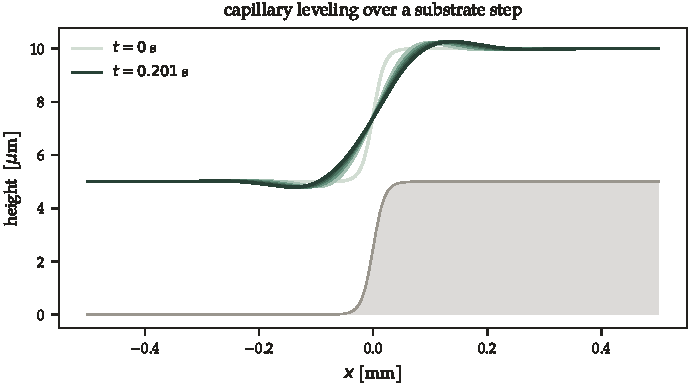
\includegraphics[width=\textwidth]{../figures/leveling-1d.pdf}
  \caption{Capillary leveling over a substrate step, from
    \file{leveling\_1d\_reg.toml}. The gray body is the substrate $s$; the
    curves are the free surface $h+s$ at six times between \SI{0}{\second} and
    \SI{0.2}{\second}, light to dark. The film starts as a layer of uniform
    thickness draped over the step and does not simply flatten: curvature
    drives liquid out of the convex shoulder into the concave foot, so a dip
    opens below the step and a rim builds above it. That pair --- a trough
    before the rise and an overshoot after it --- is the signature of the
    fourth-order leveling operator, and it is what \cref{ch:governing}
    derives.\label{fig:gallery:leveling1d}}
\end{figure}

\begin{figure}[tbp]
  \centering
  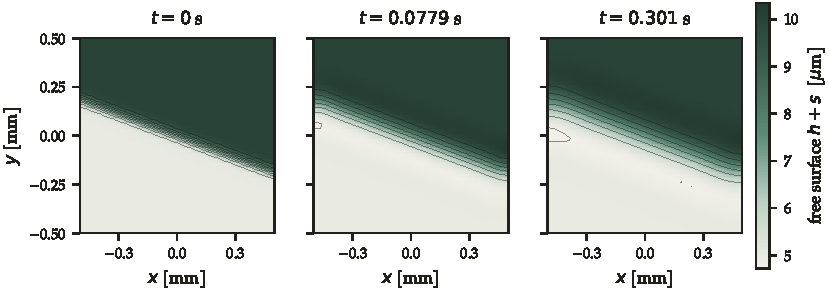
\includegraphics[width=\textwidth]{../figures/leveling-2d.pdf}
  \caption{The same physics in plan view, from \file{allphys\_2d\_reg.toml},
    which has every term switched on, including gravity in the plane and the
    centrifugal term. The color is the free surface $h+s$; the contours are
    drawn from the same field. The initial step is a straight edge crossing the
    domain obliquely, so nothing about the answer is aligned with either grid
    direction, and it spreads into a broad ramp with the trough of
    \cref{fig:gallery:leveling1d} now visible as a closed
    contour.\label{fig:gallery:leveling2d}}
\end{figure}

\section{Models}
\label{sec:intro:models}

Four combinations of dimension and concentration model are implemented. The
choice is made by two keys, \key{Physics.ConcField.Model} and
\key{Grid.Dimension}.

\begin{yzntable}{The four models\label{tab:models}}{@{}L{0.13\textwidth} L{0.13\textwidth} L{0.64\textwidth}@{}}
\textsf{\bfseries Model} & \textsf{\bfseries Dimension} & \textsf{\bfseries Description}\\ \midrule
\val{"WM"} & \val{"xh"}  & 1-D ridge, concentration uniform across the film thickness \\
\val{"WM"} & \val{"xyh"} & 2-D plan view, concentration uniform across the film thickness \\
\val{"CZ"} & \val{"xh"}  & 1-D film, concentration resolved through the thickness, $c(x,z,t)$ \\
\val{"CZ"} & \val{"xyh"} & 2-D film, concentration resolved through the thickness, $c(x,y,z,t)$ (pseudo 3-D) \\
\end{yzntable}

``Well mixed'' means the solute concentration is taken to be uniform across the
film thickness. The \val{"CZ"} model resolves it instead, at the cost of a grid
in $z$ and of two physics terms: disjoining pressure and the source term are
not available there, so contact-line problems must use \val{"WM"}.
\Cref{ch:concentration} compares the two and says when the well-mixed
assumption fails.

\section{How the pieces fit together}
\label{sec:intro:pieces}

A Yuzen run is a single process reading a single input file. \textbf{One
process on one machine} --- Yuzen is parallelized with OpenMP and has no MPI
support, so the size of problem you can solve is bounded by the memory of one
node (\cref{ch:parallel}).

\begin{enumerate}
  \item The input file, a TOML document, is parsed and checked for
        consistency. An inconsistent input aborts the run before any
        computation starts.
  \item The dimensional input is converted to the internal dimensionless form.
        The scales actually used are printed in the run log on standard
        output.
  \item A result directory named after \key{JobName} is created, and the input
        file is copied into it, so a result directory is self-describing.
  \item The solver advances the film height with a Newton--Kantorovich
        iteration, solving the concentration equation inside the same
        iteration, until the end time is reached, the film dries out, or the
        solution goes steady.
  \item Fields, history and per-step diagnostics are written at independent
        intervals.
\end{enumerate}

The height equation is advanced with Crank--Nicolson in time and an analytic
Jacobian assembled term by term; the concentration equation is solved
semi-implicitly inside the Newton loop, so that the converged state satisfies
both equations simultaneously (\cref{sec:time:coupling}). The time step adapts
from a local truncation error estimate. Two linear-solver backends are
available behind one interface, Eigen and AMGCL (\cref{ch:linearsolver}).

\section{Reproducibility}
\label{sec:intro:repro}

Two properties are worth stating at the outset because they shape the code.

First, Yuzen returns \emph{bit-identical} results regardless of OpenMP thread
count, with the \val{"amgcl"} backend as the documented exception. The test
suite asserts this and \code{ctest} re-runs the whole suite under one and four
threads. \Cref{ch:reproducibility} explains the four implementation details
that this depends on --- and why none of them may be ``tidied up''.

Second, every number in \cref{ch:verification} is reproducible from the
repository, and the command that reproduces it is printed next to it.
\Cref{ch:notverified} lists what has not been checked.

\section{License and citation}
\label{sec:intro:license}

This manual documents Yuzen 1.0. \Cref{ch:policy} says what the version number
promises about input files and about results, and \cref{ch:revisions} lists
what this release contains.

Yuzen is distributed under the Apache License, Version 2.0; see \file{LICENSE}
and \file{NOTICE}. Bundled third-party code is doctest (MIT) and toml++ (MIT,
with one local fix); Eigen (MPL-2.0, required) and AMGCL (MIT, optional) are
fetched at build time. \file{THIRD\_PARTY\_NOTICES.md} gives their versions
and describes the change to toml++. If you use Yuzen in published work, please
cite it as given in \file{CITATION.cff}.

The code, its comments, the source documents in \file{docs/} from which
Parts~III to~V of this manual are derived, and this manual itself are all in
English.
